\documentclass[xcolor=dvipsnames]{beamer}

\usepackage{amsmath}
\usepackage{listings}
\usepackage{outlines}
\usepackage{graphicx}
\usepackage{amsfonts}
\usepackage{bbm}

\usetheme{Madrid}
\useoutertheme{miniframes} % Alternatively: miniframes, infolines, split
\useinnertheme{circles}

\definecolor{IITHorange}{RGB}{243, 130, 33} % UBC Blue (primary)
\definecolor{IITHyellow}{RGB}{254, 203, 10} % UBC Grey (secondary)

\setbeamercolor{palette primary}{bg=IITHorange,fg=white}
\setbeamercolor{palette secondary}{bg=IITHorange,fg=white}
\setbeamercolor{palette tertiary}{bg=IITHorange,fg=white}
\setbeamercolor{palette quaternary}{bg=IITHorange,fg=white}
\setbeamercolor{structure}{fg=IITHorange} % itemize, enumerate, etc
\setbeamercolor{section in toc}{fg=IITHorange} % TOC sections

% Override palette coloring with secondary
\setbeamercolor{subsection in head/foot}{bg=IITHyellow,fg=white}

\definecolor{codegreen}{rgb}{0,0.6,0}
\definecolor{codegray}{rgb}{0.5,0.5,0.5}
\definecolor{codepurple}{rgb}{0.58,0,0.82}
\definecolor{backcolour}{rgb}{0.95,0.95,0.92}

\lstdefinestyle{mystyle}{
    backgroundcolor=\color{backcolour},   
    commentstyle=\color{codegreen},
    keywordstyle=\color{magenta},
    numberstyle=\tiny\color{codegray},
    stringstyle=\color{codepurple},
    basicstyle=\ttfamily\footnotesize,
    breakatwhitespace=false,         
    breaklines=true,                 
    captionpos=b,                    
    keepspaces=true,                 
    numbers=left,                    
    numbersep=5pt,                  
    showspaces=false,                
    showstringspaces=false,
    showtabs=false,   
    tabsize=2
}
\lstset{style=mystyle}

\title[Report 03/05]{Report 03/05}

\begin{document}
	
	\begin{frame}
		\titlepage
	\end{frame}
	

	\section{Introduction}

	\begin{frame}{Introduction}
        This presentation shows a summary of the work done in the past few weeks. It includes the models used and the results obtained.
        

        \textit{This document is for internal use, so it may contain some errors.}

	\end{frame}

    \section{Models}


    \begin{frame}{Models}

        \begin{itemize}
            \item Naive (nv)
            \item Naive 2.0 (nv2)
            \item KNNR + GA algorithm (knnr)
            \item KNN regression (knnreg)
        \end{itemize}

    \end{frame}

    \begin{frame}{Naives}

        Naive:

        \begin{equation}\label{eq:naive}
            y_{ih} = \beta_0 + \beta_{1h} + \beta_{2m} + \beta_3*avg\_sfcWind + \beta_{4h}*avg\_sfcWind + \epsilon_i 
        \end{equation}

        Naive 2.0:

        \vspace{0.5em}

        \qquad Adds to Equation \ref{eq:naive} the following terms:

        \begin{equation}
            \begin{split}
                & \beta_5*prev\_avg\_sfcWind + \beta_{6}*nxt\_avg\_sfcWind \\
                &  +  \beta_{7h}*prev\_avg\_sfcWind +  \beta_{8h}*nxt\_avg\_sfcWind + \epsilon_i 
            \end{split}
        \end{equation}
                        
    

    \end{frame}

    \begin{frame}{Other algorithms}
        \begin{outline}
            \1 KNNR + GA algorithm (knnr)
              \2 We implement the algorithm showed in Taesam Lee and Changsam Jeong (2014) paper.
              \2 As we are using a GA algorithm, it's necessary to run the algorithm many times to get a stable result. We run the algorithm 10 times. The probability of crossover was 0.3. We need to discuss about the mutation step.
            \1 KNN regression
                \2 We don't adjust the hyperparameters. Number of neighbors and the weight function were fixed. Also we don't use the month as a possible predictor.
           \end{outline}
  
    \end{frame}

    \section{Results}

    \subsection{Series}

    \begin{frame}
        \begin{figure}
            \centering
                 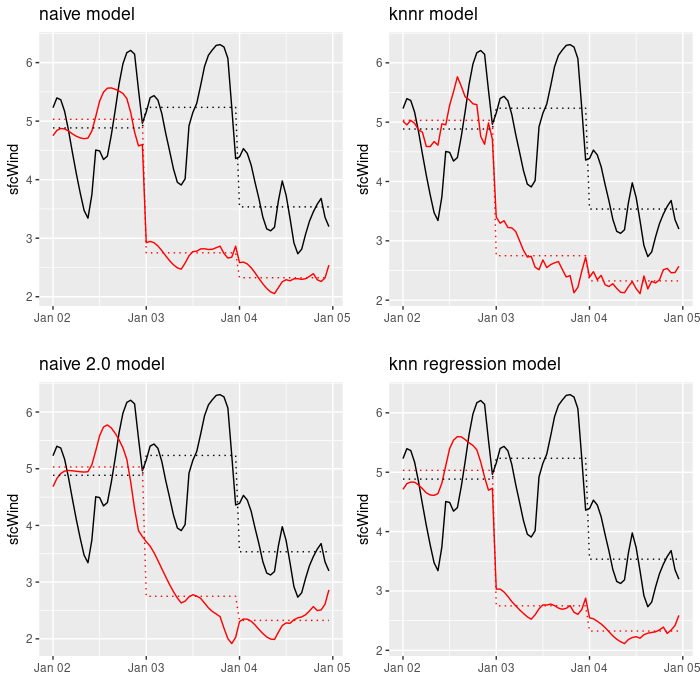
\includegraphics[width=0.57\textwidth]{images/series.png}
            \label{fig:series}
        \end{figure}
    \end{frame}

    \begin{frame}{Comments}
        \begin{outline}
            \1 There is a difference between the average value of the day of the real and the cmip data.
            \1 We can see that serie has a different behavior in the reanalysis data and the downscaled data.
                \2 In all the models the amplitude of the series seems smaller than the amplitude of the reanalysis data.
                \2 The models seem to have a bias in the prediction of the peaks (and valleys).
           \end{outline}
    \end{frame}

    \subsection{Metrics}
    \begin{frame}{}
        \scalebox{0.85}{
        
            \centering
            \begin{tabular}{|l|c|c|c|c|c|c|}
            \hline
            & diff\_of\_means & ratio\_of\_sd & ks\_test & amp\_rtio\_means & max\_error & sign\_cor \\
            \hline
            nv & 0.240 & 0.840 & 0 & 0.322 & 0.488 & 0.265 \\
            knnr & 0.240 & 0.861 & 0 & 0.554 & 0.210 & 0.040 \\
            nv\_2 & 0.240 & 0.863 & 0 & 0.523 & 0.344 & 0.175 \\
            knnreg & 0.236 & 0.828 & 0 & 0.342 & 0.313 & 0.205 \\
            \hline
            \end{tabular}
        }
    \end{frame}

    \begin{frame}{Comments 1/2}
        \begin{outline}
            \1 $diff\_of\_means = \bar{Y} - \bar{\hat{Y}}$
            \1 $ratio\_of\_sd = \frac{\sigma_{\hat{Y}}}{\sigma_{Y}}$    
            \1 $ks\_test$ is the p-value of the Kolmogorov-Smirnov test
            \1 $amp\_rtio\_means = \sum_{d=1}^{n}\frac{max({y \in D_d}) - min({y \in D_d})}{max({\hat{y} \in D_d}) - min({\hat{y} \in D_d})}$
            \1 $max\_error = \frac{\sum_{h=1}^{24}\#maximum_h(Y) - \#maximum_h(\hat{Y})}{2n}$
            \1 $sign\_cor = \frac{\sum_{h=1}^{24}(\sum_{i \in N_h}\mathbbm{1}(y_i > y_{i+1}) - \sum_{i \in N_h}\mathbbm{1}(\hat{y}_i > \hat{y}_{i+1}))}{24n}$    
        \end{outline}
    \end{frame}

    \begin{frame}{Comments 2/2}
        \begin{outline}
            \1 $n$: Number of days
            \1 $D_d$: Day $d$
            \1 $maximum_h(Y)$: Returns the days where the maximum of the day is at hour $h$
            \1 $N_h = \{h + 24z: z \in {1, \ldots, n}\}$
        \end{outline}
    \end{frame}

    \subsection{How Often Peaks Hit Hourly}
    \begin{frame}{}
        \begin{figure}
            \centering
                 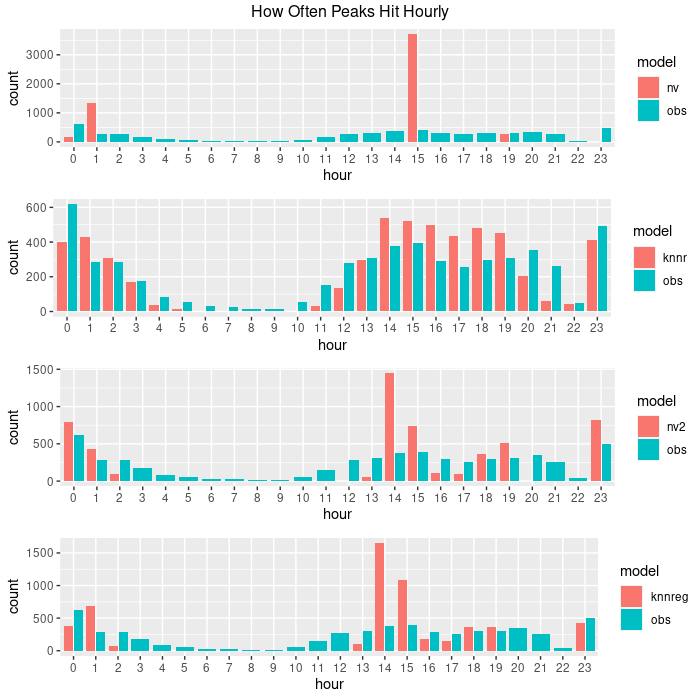
\includegraphics[width=0.57\textwidth]{images/hourly.png}
       \end{figure}
    \end{frame}
    \begin{frame}{Comments}
        \begin{outline}
            \1 On this aspect the worst model is the naive model since practically predict all the peaks in the same hour.
                \2 The naive 2.0 is a improvement of the naive model on this aspect, but seems that is not good enough.
            \1 The knnr is the one with best performance. Besides some differences predict peaks at different hours.
        \end{outline}
        
    \end{frame}

    \subsection{Densities}
    \begin{frame}{}
        \begin{figure}
            \centering
                 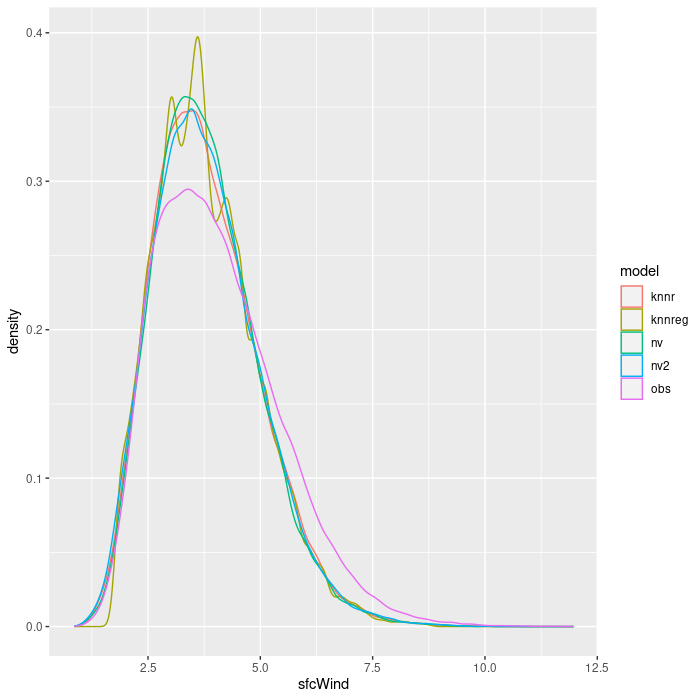
\includegraphics[width=0.57\textwidth]{images/densities.png}
       \end{figure}
    \end{frame}
    \begin{frame}{Comments}
        \begin{outline}
            \1 The downscaled distribution of all the models is more concentrated over the mode than the reanalysis distribution.
            \1 The upper tail of the reanalysis is heavier than the downscaled distribution of all the models.
            \1 The knn regression model has a multimodal distribution that is anything like the reanalysis distribution, also gives a near zero probability to the smallest values.
        \end{outline}
    \end{frame}

    \subsection{Extremograms}
    \begin{frame}{}
        \begin{figure}
            \centering
                 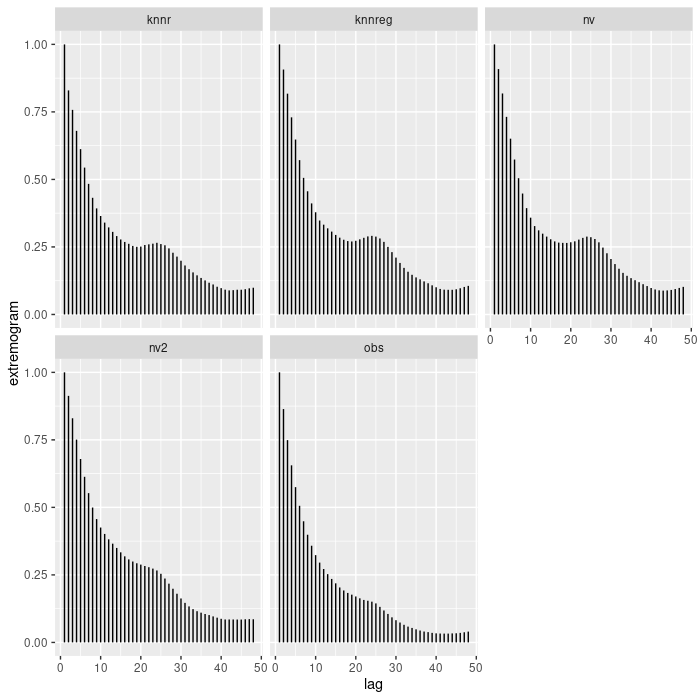
\includegraphics[width=0.57\textwidth]{images/extremograms.png}
       \end{figure}
    \end{frame}
    \begin{frame}{Comments}
        \begin{outline}
            \1 In all the models we have that the likelihood of an extreme value appearing with a large lag is consistently overestimated i.e. all the extremograms had a slower decay than the extremogram of the reanalysis.
            \1 In every model, the extremogram shows a rise around the lag 24, indicating that when an extreme value occurs, the next day is more likely to also experience an extreme value, in comparison with the reanalysis.
        \end{outline}
    \end{frame}    

    \subsection{ACF}
    \begin{frame}{}
        \begin{figure}
            \centering
                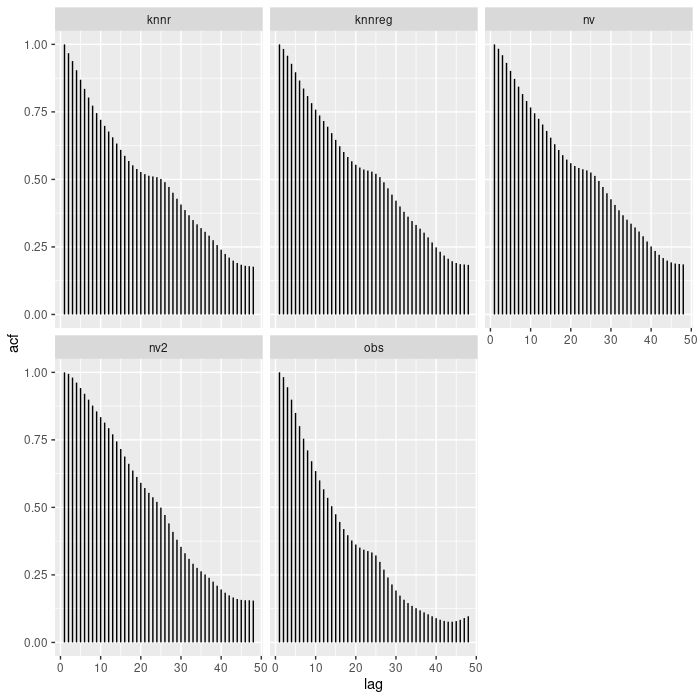
\includegraphics[width=0.57\textwidth]{images/acf.png}
       \end{figure}
    \end{frame}

    \begin{frame}{Comments}
        \begin{outline}
            \1 The reanalysis acf plot has a considerable steepest decay
            \1 An interest result that I don't here is the acf by hour, there we can see that for the hour that are different of the 0 hour the acf is overestimated and for the 0 hour the acf is underestimated.
        \end{outline}
    \end{frame}   

\end{document}
